
\documentclass[xcolor={dvipsnames}]{beamer}
\usepackage{amsmath}
% \usepackage{beamerthemesplit} // Activate for custom appearance
\usepackage{hyperref}
\usepackage{ragged2e}
\input xy 
\xyoption{all}
\usepackage{verbatim}

\title{K-means and\\
Hierarchical Clustering}
\author{Schwartz}
\date{\today}

\begin{document}

\frame{\titlepage}

\frame
{
 \frametitle{Best. Music. \emph{EVAR}}

\begin{columns}
\begin{column}{.55\textwidth}

 \begin{enumerate}
 \item Elliott Smith
 \item Sufjan Stevens
 \item Iron and Wine
 \item Damien Rice
 \end{enumerate}


\begin{enumerate}
\item Die Antwoord
\item Kendrick Lamar
\item Dan le Sac Vs Scroobius Pip
%Ry Legit \item Emalkay
%\item Skrillex FuntCase, 
 \end{enumerate}


\begin{enumerate}
 \item Rufus Wainwright
 \item Lyle Lovett
\item  Julie Doiron
%\item Our Lady Peace
% \item Eve Six
% \item Better than Ezra
 %Lit
%$Sum 41
% \item Johnny Q. Public
 \end{enumerate}


\end{column}


\begin{column}{.55\textwidth}


 \begin{enumerate}
 \item D'Gary
 \item Kishi Bashi
 \item Christine and the Queens
 \item Beirut 
 %\item Cake
 %\item Beastie Boys
 \end{enumerate}


 \begin{enumerate}
 \item Rage Against the Machine
 \item System of a Down
 \item Smashing Pumpkins
%\item Jimmy Eat World
%\item Bush
 \end{enumerate}

 \begin{enumerate}
 \item Beck
\item Cake
\item Beastie Boys
%\item Smash Mouth
\end{enumerate}

\end{column}
\end{columns}


%\includegraphics[width=3.65in]{stuffs/biodiversity.jpg}
}



\frame
{
 \frametitle{Objectives}
\begin{itemize}
\item \textcolor{gray}{Review \emph{Supervised} versus \emph{Unsupervised}}
\item $K$-means (not to be confused with $KNN$)
\begin{itemize}
\item \textcolor{gray}{and the curse of dimensionality}
\item \textcolor{gray}{\emph{norms} and the curse of dimensionality}
\item \textcolor{gray}{more about the curse of dimensionality}
\end{itemize}
\item Choosing $K$
\begin{itemize}
\item Elbow, Silhouette, and Gap methods
\end{itemize}
\item Hierarchical clustering
\item DBSCAN  
\item Bayesian mixture models
\item Expectation-Maximization (EM) algorithm  
 \end{itemize}

}



\frame
{
 \frametitle{ML Cosmology}

\vspace{-2.5em} 
\hspace*{-1.5em} \xymatrix{
 &  \txt{Learning} \ar[d] \\
\txt{\textcolor{white}{Optimization}\\\textcolor{white}{(Gradient Descent)}} & \txt{\textbf{Supervised}} \ar[dl] \ar[d]& \txt{\textcolor{white}{\textbf{Unsupervised}}} \\
Regression   &  Classification  & \txt{\textcolor{white}{\textbf{K-means}}\\\textcolor{white}{\textbf{Hierarchical}}\\\textcolor{white}{\textbf{Clustering, PCA}}\\\textcolor{white}{\textbf{...}}}\\
\txt{\textcolor{white}{Nonparametric}\\\textcolor{white}{{Decision Tree}}\\\textcolor{white}{{SVM}, KNN}} & \txt{\textcolor{white}{Parametric}\\\textcolor{white}{{Linear Models}}\\\textcolor{white}{{Bayesian}, Nets}} &  \\
\txt{\textcolor{white}{{Regularization}}\\\textcolor{white}{{Cross Validation}}} & \txt{\textcolor{white}{Boosting, Bagging}\\\textcolor{white}{Random e.g. Forests}}  & \txt{\textcolor{white}{Continuous?}\\\textcolor{white}{Categorical}}
}
}


\frame
{
 \frametitle{ML Cosmology}

\vspace{-2.5em} 
\hspace*{-1.5em} \xymatrix{
 &  \txt{Learning} \ar[d] \\
\txt{\textcolor{white}{Optimization}\\\textcolor{white}{(Gradient Descent)}} & \txt{\textbf{Supervised}} \ar[dl] \ar[d]& \txt{\textcolor{white}{\textbf{Unsupervised}}} \\
Regression\ar[dr] \ar[d]   &  Classification \ar[d] \ar[dl]& \txt{\textcolor{white}{\textbf{K-means}}\\\textcolor{white}{\textbf{Hierarchical}}\\\textcolor{white}{\textbf{Clustering, PCA}}\\\textcolor{white}{\textbf{...}}}\\
\txt{\textcolor{gray}{Nonparametric}\\\textcolor{ForestGreen}{{Decision Tree}}\\NN\textcolor{gray}{(?)}, \textcolor{red}{KNN}} & \txt{\textcolor{gray}{Parametric}\\\textcolor{ForestGreen}{{Linear Models}}\\\textcolor{ForestGreen}{{Bayes}, \textcolor{red}{SVM}\textcolor{gray}{(?)} }}   &  \\
\txt{\textcolor{white}{{Regularization}}\\\textcolor{white}{{Cross Validation}}} & \txt{\textcolor{white}{Boosting, Bagging}\\\textcolor{white}{Random e.g. Forests}}  & \txt{\textcolor{red}{Continuous?}\\\textcolor{ForestGreen}{Categorical}}
}
}


\frame
{
 \frametitle{ML Cosmology}

\vspace{-2.5em} 
\hspace*{-1.5em} \xymatrix{
 &  \txt{Learning} \ar[d] \\
\txt{\textcolor{white}{Optimization}\\\textcolor{white}{(Gradient Descent)}} & \txt{\textbf{Supervised}} \ar[dl] \ar[d]& \txt{\textcolor{white}{\textbf{Unsupervised}}} \\
Regression\ar[dr] \ar[d]   &  Classification \ar[d] \ar[dl] & \txt{\textcolor{white}{\textbf{K-means}}\\\textcolor{white}{\textbf{Hierarchical}}\\\textcolor{white}{\textbf{Clustering, PCA}}\\\textcolor{white}{\textbf{...}}}\\
\txt{\textcolor{gray}{Nonparametric}\\\textcolor{ForestGreen}{{Decision Tree}}\\NN\textcolor{gray}{(?)}, \textcolor{red}{KNN}} & \txt{\textcolor{gray}{Parametric}\\\textcolor{ForestGreen}{{Linear Models}}\\\textcolor{ForestGreen}{{Bayes}, \textcolor{red}{SVM}\textcolor{gray}{(?)}}} &   \\
\txt{\textcolor{purple}{{Regularization}}\\\textcolor{purple}{{Cross Validation}}} \ar@{-->}[ur] \ar@{-->}[u] & \txt{\textcolor{NavyBlue}{Boosting, Bagging}\\\textcolor{NavyBlue}{Random e.g. Forests}} \ar@{-->}[ul] \ar@{-->}[u] & \txt{\textcolor{red}{Continuous?}\\\textcolor{ForestGreen}{Categorical}}
}
}


\frame
{
 \frametitle{ML Cosmology}

\vspace{-2.5em} 
\hspace*{-1.5em} \xymatrix{
 &  \txt{Learning} \ar[d] \\
\txt{\textcolor{Orange}{Optimization}\\\textcolor{Orange}{(Gradient Descent)}} \ar@{<-->}[ur]& \txt{\textbf{Supervised}}\ar[dl] \ar[d]& 
 \txt{\textcolor{white}{\textbf{Unsupervised}}} \\
Regression\ar[dr] \ar[d]   &  Classification \ar[d] \ar[dl] &\txt{\textcolor{white}{\textbf{K-means}}\\\textcolor{white}{\textbf{Hierarchical}}\\\textcolor{white}{\textbf{Clustering, PCA}}\\\textcolor{white}{\textbf{...}}}\\
\txt{\textcolor{gray}{Nonparametric}\\\textcolor{ForestGreen}{{Decision Tree}}\\NN\textcolor{gray}{(?)}, \textcolor{red}{KNN}} & \txt{\textcolor{gray}{Parametric}\\\textcolor{ForestGreen}{{Linear Models}}\\\textcolor{ForestGreen}{{Bayes}, \textcolor{red}{SVM}\textcolor{gray}{(?)} }}  &   \\
\txt{\textcolor{purple}{{Regularization}}\\\textcolor{purple}{{Cross Validation}}} \ar@{-->}[ur] \ar@{-->}[u] & \txt{\textcolor{NavyBlue}{Boosting, Bagging}\\\textcolor{NavyBlue}{Random e.g. Forests}} \ar@{-->}[ul] \ar@{-->}[u] & \txt{\textcolor{red}{Continuous?}\\\textcolor{ForestGreen}{Categorical}}
}
}


\frame
{
 \frametitle{ML Cosmology}

\vspace{-2.5em} 
\hspace*{-1.5em} \xymatrix{
 &  \txt{Learning} \ar[dr] \ar[d] \\
\txt{\textcolor{Orange}{Optimization}\\\textcolor{Orange}{(Gradient Descent)}} \ar@{<-->}[ur]& \txt{\textbf{Supervised}}\ar[dl] \ar[d]& \txt{\textcolor{blue}{{\textbf{Unsupervised}}}}  \\
Regression\ar[dr] \ar[d]   &  Classification \ar[d] \ar[dl] & \txt{\textcolor{white}{\textbf{K-means}}\\\textcolor{white}{\textbf{Hierarchical}}\\\textcolor{white}{\textbf{Clustering, PCA}}\\\textcolor{white}{\textbf{...}}}\\
\txt{\textcolor{gray}{Nonparametric}\\\textcolor{ForestGreen}{{Decision Tree}}\\NN\textcolor{gray}{(?)}, \textcolor{red}{KNN}} & \txt{\textcolor{gray}{Parametric}\\\textcolor{ForestGreen}{{Linear Models}}\\\textcolor{ForestGreen}{{Bayes}, \textcolor{red}{SVM}\textcolor{gray}{(?)} }} &   \\
\txt{\textcolor{purple}{{Regularization}}\\\textcolor{purple}{{Cross Validation}}} \ar@{-->}[ur] \ar@{-->}[u] & \txt{\textcolor{NavyBlue}{Boosting, Bagging}\\\textcolor{NavyBlue}{Random e.g. Forests}} \ar@{-->}[ul] \ar@{-->}[u] & \txt{\textcolor{red}{Continuous?}\\\textcolor{ForestGreen}{Categorical}}
}
}

\frame
{
 \frametitle{ML Cosmology}

\vspace{-2.5em} 
\hspace*{-1.5em} \xymatrix{
 &  \txt{Learning} \ar[dr] \ar[d] \\
\txt{\textcolor{Orange}{Optimization}\\\textcolor{Orange}{(Gradient Descent)}} \ar@{<-->}[ur]& \txt{\textbf{Supervised}}\ar[dl] \ar[d]& \txt{\textcolor{blue}{{\textbf{Unsupervised}}}} \ar[d] \\
Regression\ar[dr] \ar[d]   &  Classification \ar[d] \ar[dl] & \txt{\textcolor{blue}{\textbf{K-means}}\\\textcolor{blue}{\textbf{Hierarchical}}\\\textcolor{blue}{\textbf{Clustering, PCA}}\\\textcolor{blue}{\textbf{... and so on ...}}}\\
\txt{\textcolor{gray}{Nonparametric}\\\textcolor{ForestGreen}{{Decision Tree}}\\NN\textcolor{gray}{(?)}, \textcolor{red}{KNN}} & \txt{\textcolor{gray}{Parametric}\\\textcolor{ForestGreen}{{Linear Models}}\\\textcolor{ForestGreen}{{Bayes}, \textcolor{red}{SVM}\textcolor{gray}{(?)} }} &   \\
\txt{\textcolor{purple}{{Regularization}}\\\textcolor{purple}{{Cross Validation}}} \ar@{-->}[ur] \ar@{-->}[u] & \txt{\textcolor{NavyBlue}{Boosting, Bagging}\\\textcolor{NavyBlue}{Random e.g. Forests}} \ar@{-->}[ul] \ar@{-->}[u] & \txt{\textcolor{red}{Continuous?}\\\textcolor{ForestGreen}{Categorical}}
}
}




\frame
{
 \frametitle{Unsupervised learning}

\vspace{-1.5em}
\begin{figure}
\centering
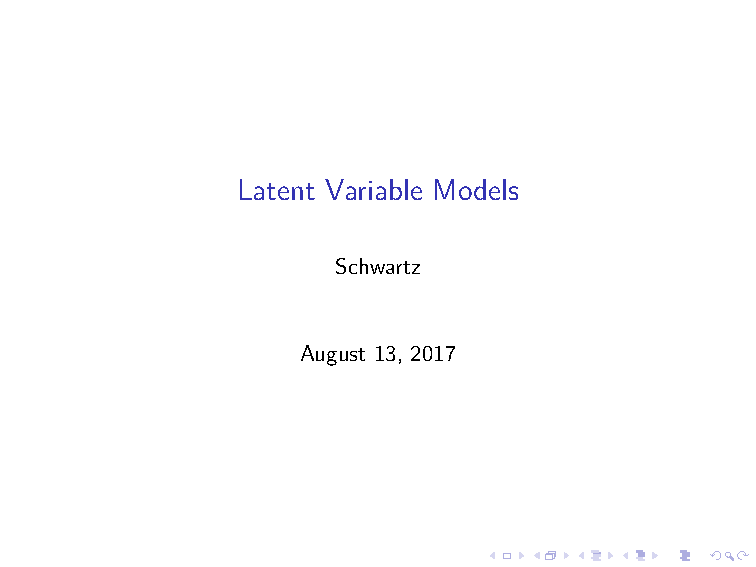
\includegraphics[width=1.87in]{stuffs/pca.png} 
\raisebox{.35em}{\includegraphics[width=2.5in]{stuffs/cluster0.png}}
\begin{tabular}{cc}
Low dimensional representations & Homogeneous subgroups \\
of data capturing data variation  & capturing data substructure\
\end{tabular}
\end{figure}

}




\frame
{
 \frametitle{Supervised versus Unsupervised}

\begin{columns}
\begin{column}{.5\textwidth}
\begin{figure}
\centering
Human Genetic Diversity in Asia
\textcolor{gray}{Two-Dimensional Representation} 
\includegraphics[width=2in]{stuffs/dna_pca.jpg}
\end{figure}
\end{column}
\begin{column}{.65\textwidth}
%\vspace{1.6em}
\begin{itemize}
\itemsep.16em 
\item[]<2-> Unsupervised learning provides
\item[]
\item<3-> \underline{exploratory data analysis (EDA)} to\\
look at/uncover feature structure
\item[]
\item<4->  \underline{anomaly detection} to provide \\ 
 data quality control (QC)
\item[]
\item<5-> \underline{dimensionality reduction} to \\
 simplify large feature spaces 
\end{itemize}
\end{column}
\end{columns}

\begin{itemize}
\item[]
\item[]<6-> ``Labels'' are sometimes used to facilitate these objectives\\
but unlike supervised learning, unsupervised learning is not 
necessarily immediately concerned with predicting outcomes\\
\textcolor{gray}{ (labels, targets, $Y$, dependent/endogenous variables)}
\end{itemize}

}


\frame
{
 \frametitle{K-Means}

\vspace{-.5em}
\begin{columns}
\begin{column}{.4\textwidth}
\begin{enumerate}
\item Choose \emph{number of clusters}, $K$
\item Randomly assign data to each cluster $k$
\item Compute the centroid for each cluster $k$
\item Assign data to the cluster with the closest centroid
\item Return to step 3, unless the centroids have stabilized
\end{enumerate}
\end{column}
\begin{column}{.7\textwidth}

${}$\\%\vspace{1em}
\includegraphics[width=2.85in]{stuffs/kmeans.png}
\end{column}
\end{columns}

\onslide<2->{\textcolor{gray}{Other init. ideas?}}

}





\frame
{
 \frametitle{K?}

\begin{figure}
\centering
\includegraphics[width=2in]{stuffs/cluster1.png}
\vspace{1.25em}
\includegraphics[width=4in]{stuffs/cluster2.png}
\end{figure}

}


\frame
{
 \frametitle{\textcolor{Maroon}{Elbow} \textcolor{gray}{and} \textcolor{NavyBlue}{Silhouette} \textcolor{gray}{methods}}
\vspace{-1.15in}
\begin{columns}
\begin{column}{.5\textwidth}
\vspace{.25em}
\color{Maroon}
For some clustering $C_K(i) \mapsto \{1,2, \cdots K\}$\\
clustering fit can be measured as 
$$W(C_K) = \frac{1}{K}\sum_{C_K(i) = C_K(j) = k} || x_i - x_j ||^2$$
\onslide<2->{
\underline{Select based on diminishing returns}}
\end{column}
\begin{column}{.53\textwidth}
\color{NavyBlue}
\onslide<3->{
$\bar \Delta^k_i$: $x_i$'s dissimilarity in cluster $k$\\
$\bar \Delta^{k'}_i$: $x_i$'s dissimilarity to cluster $k'$\\
($x_i$ in, \& closest to clusters $k, k'$)
$$Silhouette(i) = \frac{\bar \Delta^{k'}_i - \bar \Delta^k_i}{\max(\bar \Delta^{k'}_i, \bar \Delta^k_i)}$$}
\vspace{.11em}
\onslide<4->{
\underline{Compare average silhouette scores}}
\end{column}
\end{columns}

\onslide<2->{\hspace*{-1.5em}
\includegraphics[width=2.25in]{stuffs/clusterK.png}}\onslide<4->{$\;$\raisebox{.02em}{\includegraphics[width=2.3in]{stuffs/clusterK2.png}}}


\vspace{-2in}
\onslide<6->{\textcolor{gray}{Does the scaling of the $x$ matter?}}\onslide<5->{$\quad\quad$\textcolor{gray}{Interpret silhouette scores?}}

}


\frame
{
 \frametitle{\textcolor{Maroon}{Elbow} \textcolor{gray}{and} \textcolor{NavyBlue}{Silhouette} \textcolor{gray}{methods}}

\begin{figure}
\centering

\raisebox{.75em}{\includegraphics[height=1.3in]{stuffs/elbow1.png}}
\includegraphics[height=1.4in]{stuffs/elbow2.png}

\onslide<2->{
\vspace{-.5em}
\includegraphics[height=2in]{stuffs/sil1.png}
\raisebox{4em}{\includegraphics[height=.9in]{stuffs/sil2.png}}}
\end{figure}

}




\begin{frame}[fragile]
 \frametitle{The \emph{permutation test}}

\small
\begin{itemize}
\item Students enrolling for a popular class get ids $i = 1, \cdots n$.
As the class quickly fills, another section of the class is opened and students for that class are given ids $i = n+1, \cdots 2n$.
\tiny
\begin{verbatim}
id = np.array([ 1,  2,  3,  4,  5,  6,  7,  8,  9, 10, 11, 12, 13, 14, 15, 16, 17,
               18, 19, 20, 21, 22, 23, 24, 25, 26, 27, 28, 29, 30, 31, 32, 33, 34,
               35, 36, 37, 38, 39, 40, 41, 42, 43, 44, 45, 46, 47, 48, 49, 50, 51,
               52, 53, 54, 55, 56, 57, 58, 59, 60])
\end{verbatim}        
\small
\item<2-> The classes have the same tests...\\How could we test which class is doing better?

\tiny
\begin{verbatim}
score = np.array([59, 92, 93, 83, 92, 61, 84, 92, 70, 93, 76, 70, 84, 61, 75, 91, 73,
                  67, 65, 64, 75, 80, 66, 56, 62, 53, 82, 69, 85, 94, 80, 86, 97, 99,
                  77, 84, 94, 70, 80, 87, 77, 85, 95, 80, 88, 90, 85, 84, 92, 75, 83,
                  89, 76, 95, 91, 97, 80, 70, 71, 94])
\end{verbatim}        
\item<3-> If the classes are doing equally well, the index doesn't matter \\\onslide<4->{\textcolor{red}{$\iff$} We could \emph{permute} the index \textcolor{gray}{and see if it matters}}
\end{itemize}
\scriptsize
\begin{enumerate}
\color{gray}
\item<5->  Repeatedly permute the index and recalculating the test statistic each time 
\item \onslide<6->{These samples approximate the test statistic distribution under the null }
\item \onslide<7->{Compare the test statistic to this null distribution \\ to suggest how ``strange'' the actual observed test statistic is if the null is true}
\end{enumerate}

\end{frame}

\frame
{
 \frametitle{The \emph{permutation test} \textcolor{gray}{\emph{(This is my \textbf{favorite} test, btw)}}}

\begin{enumerate}
\item Permute the ids (i.e., believe the null is true: ids don't matter)
\item Recalculate the test statistic each time (under null)
\item See how strange your observed statistic is compared to nulls 
\end{enumerate}
\vspace{-.75em}
\begin{figure}
\centering
\includegraphics[width=3.75in]{stuffs/testStat_nullDist.png}
\end{figure}

}

\frame
{
 \frametitle{The \emph{permutation test} and the \emph{null distribution}}

\begin{itemize}
\item What was needed in the permutation test was really the distribution of the test statistic under the null hypothesis
\item[]
\item<2-> We used permutation to get it\\ \onslide<3->{but that was just a means to an end}
\item[]
\item<4-> We can test against \emph{ANY} null distribution we wish to propose
\end{itemize}
}

\frame
{
 \frametitle{The Gap statistic}
\small
\onslide<2->{For $M$ null distribution samples, calculate
\scriptsize 
$$\text{Gap($K$)} = \bar l  - \log W^{(*)}(C_K) \quad \text{ and } \quad s_{K} = \sqrt{\frac{1}{R} \sum_{j=1}^M \left(\log W^{(r)}(C_K) - \bar l \right)^2}$$
\vspace{-1em}
$$\text{where } W^{(r)}(C_K) = \sum_{C_K(i) = C_K(j) = k} || x_i^{(r)} - x_j^{(r)} ||^2 \quad \text{ and } \quad \bar l = \frac{1}{R} \sum_{r=1}^R \log W^{(r)}(C_K) $$}

\vspace{.5em}

\small
\onslide<1->{Then choose the smallest $K$ such that Gap($K$) $\geq$ Gap($K+1$)$ - s_{K+1}$}

\onslide<1-2>{\includegraphics[width=2.25in]{stuffs/gap1.png}\raisebox{.02em}{\includegraphics[width=2.25in]{stuffs/gap2.png}}}

\only<3->{
\vspace{-2.15in}
\begin{figure}
\centering
\includegraphics[width=3.275in]{stuffs/gapzee.png}
\end{figure}
}

}




\frame
{
 \frametitle{The Curse of Dimensionality}

\begin{figure}
\centering
Just as nearest neighbors breaks down in high dimensional space...\\
Distance based clustering breaks down in high dimensional space...\\
\onslide<2->{
\textcolor{gray}{Go see Ryan's great slides motivating \emph{The Curse of Dimensionality}\\
They're in the KNN slides\\ (THIS is the KMEANS lecture, NOT the KNN lecture)}\\${}$\\
}

\onslide<3->{
However, when we normalize a vector
(e.g., turn bag-of-words into probabilities, or make it a unit vector)
we project all vectors onto a \emph{manifold} where ``locality'' and ``neighborhoods'' make sense again.

\begin{figure}
\centering
\includegraphics[width=1.5in]{stuffs/NormalizingVectors.jpg}\raisebox{.85em}{\includegraphics[width=1.5in]{stuffs/3D_Direction_Vectors.png}}
\end{figure}
}


\end{figure}

}



\frame
{
 \frametitle{The Curse of Dimensionality}

\vspace{.1in}

\begin{figure}
\centering

So who is effected by \emph{The Curse of Dimensionality} and \emph{why (not)?}

\end{figure}


\vspace{1.65in}

\color{gray}
Hint: \emph{Overfitting} and \\ 
\textcolor{white}{Hint: }\emph{The Curse of Dimensionality} are \\
\textcolor{white}{Hint: }slightly different things... 



}



\frame
{
 \frametitle{Challenge}

\includegraphics[width=4in]{stuffs/hier1.png}
}



\frame
{
 \frametitle{Hierarchical clustering }

\includegraphics[width=4in]{stuffs/hier2.png}


\begin{columns}
\scriptsize
\begin{column}{.5\textwidth}

\begin{enumerate}
\item Assign each point to it's own cluster
\item<2-> Computer pairwise cluster distances
\item<3-> Merge \emph{closest two} clusters
\item<4-> Return to 2 until all clusters merged
\end{enumerate}
\end{column}
\begin{column}{.7\textwidth}
\begin{itemize}
\setlength\itemsep{.5em}
\item<5> Single:  minimum pairwise point dissimilarity 
\item<5> Complete: maximum pairwise point dissimilarity 
\item<5> Average:  average pairwise point dissimilarity 
\item<5> Centroid:  centroid dissimilarity 
\end{itemize}

\end{column}
\end{columns}

\vspace{-.8in}
\hspace{2.1in}\only<1-6>{\vspace{8em}}\only<6>{\includegraphics[width=2in]{stuffs/distance1.png}}\only<7->{\includegraphics[width=2in]{stuffs/distance2.png}}\only<7->{\vspace{2em}}

}



\frame
{
 \frametitle{Hierarchical clustering}
 
Clusterings are created based on distance between proposed merges\\${}$\\

And then the number of clusters can be chosen \emph{just like} $K$-means...


\hspace*{-2.25em}\includegraphics[width=3.075in]{stuffs/hierK.png}$\;\;$\onslide<2->{\raisebox{1.5em}{\includegraphics[width=1.75in]{stuffs/spin_colon.jpg}}}



\onslide<2->{
This is super cool, but \\
\color{red}unlike $K$-means, hierarchical clustering requires all pairwise 
comparisons so it doesn't scale gracefully with increasing data...}

}





\frame
{
 \frametitle{DBSCAN}

\begin{columns}
\begin{column}{.4\textwidth}
\includegraphics[width=1.75in]{stuffs/kmeanstrap.png}

\hspace*{1em}\onslide<6->{\includegraphics[width=1.75in]{stuffs/db3.png}}
\end{column}
\begin{column}{.65\textwidth}

\vspace{-1em}
\begin{itemize}
\item<2-> Specify connection distance $\epsilon$ and minimum number of points for core $m$
\item[]
\item<3-> A cluster is all connected \emph{core points}
\item[]
\item<4-> All other points are \emph{noise}
\item[]
\item[]
\onslide<5->{\includegraphics[width=2.5in]{stuffs/db1.png}}
\item[]
\end{itemize}

\end{column}
\end{columns}


}

\frame
{
 \frametitle{DBSCAN}

\begin{figure}
\centering
\includegraphics[width=4in]{stuffs/db2.png}
\end{figure}

}



\frame
{
 \frametitle{Bayesian Mixture Models \textcolor{gray}{\emph{(xtra: my grad school jam)}}}

\vspace{-1em}
\begin{columns}
\begin{column}{.6\textwidth}

$$ f(X_i|\boldsymbol{\mu},\boldsymbol{\sigma^2}, \boldsymbol{\pi}, \boldsymbol{\pi}) = \sum_{k=1}^{K} \pi_k N(\mu_k,\sigma^2_k)$$

\end{column}
\begin{column}{.5\textwidth}

\vspace{1em}
\includegraphics[height=.5in, width=2in]{stuffs/mixt.png} 
\end{column}
\end{columns}

\vspace{-.5em}

\onslide<2->{
\begin{columns}
\begin{column}{.5\textwidth}
\begin{align*}
f(X_i|V_i,\boldsymbol{\mu},\boldsymbol{\sigma^2}, \boldsymbol{\pi}) = {}& N(\mu_k,\sigma^2_k) \\
\Pr(\boldsymbol{V}_i) = {}& Multinomial(\boldsymbol{\pi},n=1) \\
f(\boldsymbol{\pi}) = {}& Dirichlet(\boldsymbol{\omega}) \\
f(\mu_k) = {}& N(\mu_0,\sigma^2_0) \\
f(\sigma^{-2}_k) = {}& Gamma(\alpha,\beta) \\
\end{align*}
\end{column}
\begin{column}{.5\textwidth}
\small
\xymatrix{
\omega  \\
 \pi \ar[u]  &\mu_0,\sigma_0^2& \alpha,\beta\\
V_i=k  \ar[u] &\mu_k \ar[u] &  \ar[u] \sigma_k\\
 & X_i \ar[ur] \ar[ul] \ar[u]
}
\end{column}
\end{columns}}
\vspace{-.5em}
\scriptsize
\onslide<3->{$\displaystyle 
f(\mathbf{X},\mathbf{V},\boldsymbol{\mu},\boldsymbol{\sigma^2}, \boldsymbol{\pi}|\mu_0,\sigma_0^2,\alpha,\beta,\boldsymbol\omega) = 
\prod_{i=1}^n \left[ \left(\sum_{k=1}^K 1_{[V_{ik}=1]}\frac{1}{\sqrt{2\pi}\sigma_k} e^{-\frac{1}{2}\left(\frac{X_i - \mu_k}{\sigma_k}\right)^2}\right) \left(\prod_{k=1}^K \pi_k^{V_{ik}}\right)\right]$\\
$\quad\quad\quad\;\displaystyle \times \left(\prod_{k=1}^K \frac{1}{\sqrt{2\pi}\sigma_0} e^{-\frac{1}{2}\left(\frac{\mu_k - \mu_0}{\sigma_0}\right)^2} \frac{\beta^\alpha}{\Gamma(\alpha)} \left(\frac{1}{\sigma^{2}}\right)^{\alpha -1} e^{-\beta\frac{1}{\sigma^{2}}} \right) \left(\frac{1}{\mathbf{B}(\omega)}\prod_{k=1}^K \pi_k^{\omega_{k}-1}\right) $}

}


\frame
{
 \frametitle{Markov Chain Monte Carlo (MCMC) \emph{posterior sampling}}

A Gibbs sampler for the posterior 
\footnotesize
\begin{align*}
{} & f(\mathbf{V},\boldsymbol{\mu},\boldsymbol{\sigma^2}, \boldsymbol{\pi}|\mathbf{X},\mu_0,\sigma_0^2,\alpha,\beta,\boldsymbol\omega) \\
\onslide<2->{\propto{} & \textcolor{NavyBlue}{f(\mathbf{X},\mathbf{V},\boldsymbol{\mu},\boldsymbol{\sigma^2}, \boldsymbol{\pi}|\mu_0,\sigma_0^2,\alpha,\beta,\boldsymbol\omega) \quad\text{\tiny \textcolor{gray}{(which is proportional to the joint distribution)}}}}\\
{} & \onslide<3->{\text{\textcolor{gray}{Is made by cycling through the \emph{full conditional distributions}}}}
\\\\
{} & \onslide<4->{f(\mu_k|\mathbf{V},\boldsymbol{\sigma^2},\mathbf{X},\mu_0,\sigma_0^2,\alpha,\beta,\boldsymbol\omega)} \\
\onslide<5->{\propto}{} & \onslide<5->{\textcolor{NavyBlue}{f(\mathbf{X},\mathbf{V},\boldsymbol{\mu},\boldsymbol{\sigma^2}, \boldsymbol{\pi}|\mu_0,\sigma_0^2,\alpha,\beta,\boldsymbol\omega)\quad\text{\tiny \textcolor{gray}{(which is proportional to the joint distribution)}}}}\\\\
{} & \onslide<6->{f(\sigma^2_k|\mathbf{V},\boldsymbol{\sigma^2},\mathbf{X},\mu_0,\sigma_0^2,\alpha,\beta,\boldsymbol\omega)} \\
\onslide<7->{\propto}{} & \onslide<7->{\textcolor{NavyBlue}{f(\mathbf{X},\mathbf{V},\boldsymbol{\mu},\boldsymbol{\sigma^2}, \boldsymbol{\pi}|\mu_0,\sigma_0^2,\alpha,\beta,\boldsymbol\omega)\quad\text{\tiny \textcolor{gray}{(which is proportional to the joint distribution)}}}}\\\\
{} & \onslide<8->{\textcolor{black}{\Pr(V_{ik}=1|\mathbf{X},\boldsymbol{\mu},\boldsymbol{\sigma^2}, \boldsymbol{\pi},\mu_0,\sigma_0^2,\alpha,\beta,\boldsymbol\omega)}} \\
\onslide<9->{\propto}{} & \onslide<9->{\textcolor{NavyBlue}{f(\mathbf{X},\mathbf{V},\boldsymbol{\mu},\boldsymbol{\sigma^2}, \boldsymbol{\pi}|\mu_0,\sigma_0^2,\alpha,\beta,\boldsymbol\omega)\quad\text{\tiny \textcolor{gray}{(which is proportional to the joint distribution)}}}}\\\\
{} & \onslide<10->{\textcolor{black}{\Pr(\boldsymbol{\pi}|\mathbf{X},\mathbf{V},\boldsymbol{\mu},\boldsymbol{\sigma^2}, \mu_0,\sigma_0^2,\alpha,\beta,\boldsymbol\omega)}} \\
\onslide<11->{\propto}{} & \onslide<11->{\textcolor{NavyBlue}{f(\mathbf{X},\mathbf{V},\boldsymbol{\mu},\boldsymbol{\sigma^2}, \boldsymbol{\pi}|\mu_0,\sigma_0^2,\alpha,\beta,\boldsymbol\omega)\quad\text{\tiny \textcolor{gray}{(which is proportional to the joint distribution)}}}}
\end{align*}

}


\frame
{
 \frametitle{Markov Chain Monte Carlo (MCMC) \emph{posterior sampling}}

A Gibbs sampler for the posterior 
\footnotesize
\begin{align*}
{} & f(\mathbf{V},\boldsymbol{\mu},\boldsymbol{\sigma^2}, \boldsymbol{\pi}|\mathbf{X},\mu_0,\sigma_0^2,\alpha,\beta,\boldsymbol\omega) \\
\onslide<1->{\propto{} & f(\mathbf{X},\mathbf{V},\boldsymbol{\mu},\boldsymbol{\sigma^2}, \boldsymbol{\pi}|\mu_0,\sigma_0^2,\alpha,\beta,\boldsymbol\omega) \quad\text{\tiny \textcolor{gray}{(which is proportional to the joint distribution)}}}\\
{} & \onslide<1->{\text{\textcolor{gray}{Is made by cycling through the \emph{full conditional distributions}}}}
\\\\
{} & \onslide<1->{\textcolor{red}{f(\mu_k|\mathbf{V},\boldsymbol{\sigma^2},\mathbf{X},\mu_0,\sigma_0^2,\alpha,\beta,\boldsymbol\omega)}} \\
\onslide<1->{\propto}{} & \onslide<1->{\textcolor{NavyBlue}{f(\mathbf{X},\mathbf{V},\boldsymbol{\mu},\boldsymbol{\sigma^2}, \boldsymbol{\pi}|\mu_0,\sigma_0^2,\alpha,\beta,\boldsymbol\omega)\quad\text{\tiny \textcolor{gray}{(which is proportional to the joint distribution)}}}}\\\\
{} & \onslide<1->{\textcolor{black}{f(\sigma^2_k|\mathbf{V},\boldsymbol{\sigma^2},\mathbf{X},\mu_0,\sigma_0^2,\alpha,\beta,\boldsymbol\omega)}} \\
\onslide<1->{\propto}{} & \onslide<1->{\textcolor{NavyBlue}{f(\mathbf{X},\mathbf{V},\boldsymbol{\mu},\boldsymbol{\sigma^2}, \boldsymbol{\pi}|\mu_0,\sigma_0^2,\alpha,\beta,\boldsymbol\omega)\quad\text{\tiny \textcolor{gray}{(which is proportional to the joint distribution)}}}}\\\\
{} & \onslide<1->{\textcolor{black}{\Pr(V_{ik}=1|\mathbf{X},\boldsymbol{\mu},\boldsymbol{\sigma^2}, \boldsymbol{\pi},\mu_0,\sigma_0^2,\alpha,\beta,\boldsymbol\omega)}} \\
\onslide<1->{\propto}{} & \onslide<1->{\textcolor{NavyBlue}{f(\mathbf{X},\mathbf{V},\boldsymbol{\mu},\boldsymbol{\sigma^2}, \boldsymbol{\pi}|\mu_0,\sigma_0^2,\alpha,\beta,\boldsymbol\omega)\quad\text{\tiny \textcolor{gray}{(which is proportional to the joint distribution)}}}}\\\\
{} & \onslide<1->{\textcolor{black}{\Pr(\boldsymbol{\pi}|\mathbf{X},\mathbf{V},\boldsymbol{\mu},\boldsymbol{\sigma^2}, \mu_0,\sigma_0^2,\alpha,\beta,\boldsymbol\omega)}} \\
\onslide<1->{\propto}{} & \onslide<1->{\textcolor{NavyBlue}{f(\mathbf{X},\mathbf{V},\boldsymbol{\mu},\boldsymbol{\sigma^2}, \boldsymbol{\pi}|\mu_0,\sigma_0^2,\alpha,\beta,\boldsymbol\omega)\quad\text{\tiny \textcolor{gray}{(which is proportional to the joint distribution)}}}}
\end{align*}
}

\frame
{
 \frametitle{Markov Chain Monte Carlo (MCMC) \emph{posterior sampling}}

A Gibbs sampler for the posterior 
\footnotesize
\begin{align*}
{} & f(\mathbf{V},\boldsymbol{\mu},\boldsymbol{\sigma^2}, \boldsymbol{\pi}|\mathbf{X},\mu_0,\sigma_0^2,\alpha,\beta,\boldsymbol\omega) \\
\onslide<1->{\propto{} & f(\mathbf{X},\mathbf{V},\boldsymbol{\mu},\boldsymbol{\sigma^2}, \boldsymbol{\pi}|\mu_0,\sigma_0^2,\alpha,\beta,\boldsymbol\omega) \quad\text{\tiny \textcolor{gray}{(which is proportional to the joint distribution)}}}\\
{} & \onslide<1->{\text{\textcolor{gray}{Is made by cycling through the \emph{full conditional distributions}}}}
\\\\
{} & \onslide<1->{\textcolor{black}{f(\mu_k|\mathbf{V},\boldsymbol{\sigma^2},\mathbf{X},\mu_0,\sigma_0^2,\alpha,\beta,\boldsymbol\omega)}} \\
\onslide<1->{\propto}{} & \onslide<1->{\textcolor{NavyBlue}{f(\mathbf{X},\mathbf{V},\boldsymbol{\mu},\boldsymbol{\sigma^2}, \boldsymbol{\pi}|\mu_0,\sigma_0^2,\alpha,\beta,\boldsymbol\omega)\quad\text{\tiny \textcolor{gray}{(which is proportional to the joint distribution)}}}}\\\\
{} & \onslide<1->{\textcolor{red}{f(\sigma^2_k|\mathbf{V},\boldsymbol{\sigma^2},\mathbf{X},\mu_0,\sigma_0^2,\alpha,\beta,\boldsymbol\omega)}} \\
\onslide<1->{\propto}{} & \onslide<1->{\textcolor{NavyBlue}{f(\mathbf{X},\mathbf{V},\boldsymbol{\mu},\boldsymbol{\sigma^2}, \boldsymbol{\pi}|\mu_0,\sigma_0^2,\alpha,\beta,\boldsymbol\omega)\quad\text{\tiny \textcolor{gray}{(which is proportional to the joint distribution)}}}}\\\\
{} & \onslide<1->{\textcolor{black}{\Pr(V_{ik}=1|\mathbf{X},\boldsymbol{\mu},\boldsymbol{\sigma^2}, \boldsymbol{\pi},\mu_0,\sigma_0^2,\alpha,\beta,\boldsymbol\omega)}} \\
\onslide<1->{\propto}{} & \onslide<1->{\textcolor{NavyBlue}{f(\mathbf{X},\mathbf{V},\boldsymbol{\mu},\boldsymbol{\sigma^2}, \boldsymbol{\pi}|\mu_0,\sigma_0^2,\alpha,\beta,\boldsymbol\omega)\quad\text{\tiny \textcolor{gray}{(which is proportional to the joint distribution)}}}}\\\\
{} & \onslide<1->{\textcolor{black}{\Pr(\boldsymbol{\pi}|\mathbf{X},\mathbf{V},\boldsymbol{\mu},\boldsymbol{\sigma^2}, \mu_0,\sigma_0^2,\alpha,\beta,\boldsymbol\omega)}} \\
\onslide<1->{\propto}{} & \onslide<1->{\textcolor{NavyBlue}{f(\mathbf{X},\mathbf{V},\boldsymbol{\mu},\boldsymbol{\sigma^2}, \boldsymbol{\pi}|\mu_0,\sigma_0^2,\alpha,\beta,\boldsymbol\omega)\quad\text{\tiny \textcolor{gray}{(which is proportional to the joint distribution)}}}}
\end{align*}
}

\frame
{
 \frametitle{Markov Chain Monte Carlo (MCMC) \emph{posterior sampling}}

A Gibbs sampler for the posterior 
\footnotesize
\begin{align*}
{} & f(\mathbf{V},\boldsymbol{\mu},\boldsymbol{\sigma^2}, \boldsymbol{\pi}|\mathbf{X},\mu_0,\sigma_0^2,\alpha,\beta,\boldsymbol\omega) \\
\onslide<1->{\propto{} & f(\mathbf{X},\mathbf{V},\boldsymbol{\mu},\boldsymbol{\sigma^2}, \boldsymbol{\pi}|\mu_0,\sigma_0^2,\alpha,\beta,\boldsymbol\omega) \quad\text{\tiny \textcolor{gray}{(which is proportional to the joint distribution)}}}\\
{} & \onslide<1->{\text{\textcolor{gray}{Is made by cycling through the \emph{full conditional distributions}}}}
\\\\
{} & \onslide<1->{\textcolor{black}{f(\mu_k|\mathbf{V},\boldsymbol{\sigma^2},\mathbf{X},\mu_0,\sigma_0^2,\alpha,\beta,\boldsymbol\omega)}} \\
\onslide<1->{\propto}{} & \onslide<1->{\textcolor{NavyBlue}{f(\mathbf{X},\mathbf{V},\boldsymbol{\mu},\boldsymbol{\sigma^2}, \boldsymbol{\pi}|\mu_0,\sigma_0^2,\alpha,\beta,\boldsymbol\omega)\quad\text{\tiny \textcolor{gray}{(which is proportional to the joint distribution)}}}}\\\\
{} & \onslide<1->{\textcolor{black}{f(\sigma^2_k|\mathbf{V},\boldsymbol{\sigma^2},\mathbf{X},\mu_0,\sigma_0^2,\alpha,\beta,\boldsymbol\omega)}} \\
\onslide<1->{\propto}{} & \onslide<1->{\textcolor{NavyBlue}{f(\mathbf{X},\mathbf{V},\boldsymbol{\mu},\boldsymbol{\sigma^2}, \boldsymbol{\pi}|\mu_0,\sigma_0^2,\alpha,\beta,\boldsymbol\omega)\quad\text{\tiny \textcolor{gray}{(which is proportional to the joint distribution)}}}}\\\\
{} & \onslide<1->{\textcolor{red}{\Pr(V_{ik}=1|\mathbf{X},\boldsymbol{\mu},\boldsymbol{\sigma^2}, \boldsymbol{\pi},\mu_0,\sigma_0^2,\alpha,\beta,\boldsymbol\omega)}} \\
\onslide<1->{\propto}{} & \onslide<1->{\textcolor{NavyBlue}{f(\mathbf{X},\mathbf{V},\boldsymbol{\mu},\boldsymbol{\sigma^2}, \boldsymbol{\pi}|\mu_0,\sigma_0^2,\alpha,\beta,\boldsymbol\omega)\quad\text{\tiny \textcolor{gray}{(which is proportional to the joint distribution)}}}}\\\\
{} & \onslide<1->{\textcolor{black}{\Pr(\boldsymbol{\pi}|\mathbf{X},\mathbf{V},\boldsymbol{\mu},\boldsymbol{\sigma^2}, \mu_0,\sigma_0^2,\alpha,\beta,\boldsymbol\omega)}} \\
\onslide<1->{\propto}{} & \onslide<1->{\textcolor{NavyBlue}{f(\mathbf{X},\mathbf{V},\boldsymbol{\mu},\boldsymbol{\sigma^2}, \boldsymbol{\pi}|\mu_0,\sigma_0^2,\alpha,\beta,\boldsymbol\omega)\quad\text{\tiny \textcolor{gray}{(which is proportional to the joint distribution)}}}}
\end{align*}
}

\frame
{
 \frametitle{Markov Chain Monte Carlo (MCMC) \emph{posterior sampling}}

A Gibbs sampler for the posterior 
\footnotesize
\begin{align*}
{} & f(\mathbf{V},\boldsymbol{\mu},\boldsymbol{\sigma^2}, \boldsymbol{\pi}|\mathbf{X},\mu_0,\sigma_0^2,\alpha,\beta,\boldsymbol\omega) \\
\onslide<1->{\propto{} & f(\mathbf{X},\mathbf{V},\boldsymbol{\mu},\boldsymbol{\sigma^2}, \boldsymbol{\pi}|\mu_0,\sigma_0^2,\alpha,\beta,\boldsymbol\omega) \quad\text{\tiny \textcolor{gray}{(which is proportional to the joint distribution)}}}\\
{} & \onslide<1->{\text{\textcolor{gray}{Is made by cycling through the \emph{full conditional distributions}}}}
\\\\
{} & \onslide<1->{\textcolor{black}{f(\mu_k|\mathbf{V},\boldsymbol{\sigma^2},\mathbf{X},\mu_0,\sigma_0^2,\alpha,\beta,\boldsymbol\omega)}} \\
\onslide<1->{\propto}{} & \onslide<1->{\textcolor{NavyBlue}{f(\mathbf{X},\mathbf{V},\boldsymbol{\mu},\boldsymbol{\sigma^2}, \boldsymbol{\pi}|\mu_0,\sigma_0^2,\alpha,\beta,\boldsymbol\omega)\quad\text{\tiny \textcolor{gray}{(which is proportional to the joint distribution)}}}}\\\\
{} & \onslide<1->{\textcolor{black}{f(\sigma^2_k|\mathbf{V},\boldsymbol{\sigma^2},\mathbf{X},\mu_0,\sigma_0^2,\alpha,\beta,\boldsymbol\omega)}} \\
\onslide<1->{\propto}{} & \onslide<1->{\textcolor{NavyBlue}{f(\mathbf{X},\mathbf{V},\boldsymbol{\mu},\boldsymbol{\sigma^2}, \boldsymbol{\pi}|\mu_0,\sigma_0^2,\alpha,\beta,\boldsymbol\omega)\quad\text{\tiny \textcolor{gray}{(which is proportional to the joint distribution)}}}}\\\\
{} & \onslide<1->{\textcolor{black}{\Pr(V_{ik}=1|\mathbf{X},\boldsymbol{\mu},\boldsymbol{\sigma^2}, \boldsymbol{\pi},\mu_0,\sigma_0^2,\alpha,\beta,\boldsymbol\omega)}} \\
\onslide<1->{\propto}{} & \onslide<1->{\textcolor{NavyBlue}{f(\mathbf{X},\mathbf{V},\boldsymbol{\mu},\boldsymbol{\sigma^2}, \boldsymbol{\pi}|\mu_0,\sigma_0^2,\alpha,\beta,\boldsymbol\omega)\quad\text{\tiny \textcolor{gray}{(which is proportional to the joint distribution)}}}}\\\\
{} & \onslide<1->{\textcolor{red}{\Pr(\boldsymbol{\pi}|\mathbf{X},\mathbf{V},\boldsymbol{\mu},\boldsymbol{\sigma^2}, \mu_0,\sigma_0^2,\alpha,\beta,\boldsymbol\omega)}} \\
\onslide<1->{\propto}{} & \onslide<1->{\textcolor{NavyBlue}{f(\mathbf{X},\mathbf{V},\boldsymbol{\mu},\boldsymbol{\sigma^2}, \boldsymbol{\pi}|\mu_0,\sigma_0^2,\alpha,\beta,\boldsymbol\omega)\quad\text{\tiny \textcolor{gray}{(which is proportional to the joint distribution)}}}}
\end{align*}
}




\frame
{
 \frametitle{Markov Chain Monte Carlo (MCMC) \emph{posterior sampling}}

A Gibbs sampler for the posterior 
\footnotesize
\begin{align*}
{} & f(\mathbf{V},\boldsymbol{\mu},\boldsymbol{\sigma^2}, \boldsymbol{\pi}|\mathbf{X},\mu_0,\sigma_0^2,\alpha,\beta,\boldsymbol\omega) \\
\onslide<1->{\propto{} & f(\mathbf{X},\mathbf{V},\boldsymbol{\mu},\boldsymbol{\sigma^2}, \boldsymbol{\pi}|\mu_0,\sigma_0^2,\alpha,\beta,\boldsymbol\omega) \quad\text{\tiny \textcolor{gray}{(which is proportional to the joint distribution)}}}\\
{} & \onslide<1->{\text{\textcolor{gray}{Is made by cycling through the \emph{full conditional distributions}}}}
\\\\
{} & \onslide<1->{\textcolor{red}{f(\mu_k|\mathbf{V},\boldsymbol{\sigma^2},\mathbf{X},\mu_0,\sigma_0^2,\alpha,\beta,\boldsymbol\omega)}} \\
\onslide<1->{\propto}{} & \onslide<1->{\textcolor{NavyBlue}{f(\mathbf{X},\mathbf{V},\boldsymbol{\mu},\boldsymbol{\sigma^2}, \boldsymbol{\pi}|\mu_0,\sigma_0^2,\alpha,\beta,\boldsymbol\omega)\quad\text{\tiny \textcolor{gray}{(which is proportional to the joint distribution)}}}}\\\\
{} & \onslide<1->{\textcolor{black}{f(\sigma^2_k|\mathbf{V},\boldsymbol{\sigma^2},\mathbf{X},\mu_0,\sigma_0^2,\alpha,\beta,\boldsymbol\omega)}} \\
\onslide<1->{\propto}{} & \onslide<1->{\textcolor{NavyBlue}{f(\mathbf{X},\mathbf{V},\boldsymbol{\mu},\boldsymbol{\sigma^2}, \boldsymbol{\pi}|\mu_0,\sigma_0^2,\alpha,\beta,\boldsymbol\omega)\quad\text{\tiny \textcolor{gray}{(which is proportional to the joint distribution)}}}}\\\\
{} & \onslide<1->{\textcolor{black}{\Pr(V_{ik}=1|\mathbf{X},\boldsymbol{\mu},\boldsymbol{\sigma^2}, \boldsymbol{\pi},\mu_0,\sigma_0^2,\alpha,\beta,\boldsymbol\omega)}} \\
\onslide<1->{\propto}{} & \onslide<1->{\textcolor{NavyBlue}{f(\mathbf{X},\mathbf{V},\boldsymbol{\mu},\boldsymbol{\sigma^2}, \boldsymbol{\pi}|\mu_0,\sigma_0^2,\alpha,\beta,\boldsymbol\omega)\quad\text{\tiny \textcolor{gray}{(which is proportional to the joint distribution)}}}}\\\\
{} & \onslide<1->{\textcolor{black}{\Pr(\boldsymbol{\pi}|\mathbf{X},\mathbf{V},\boldsymbol{\mu},\boldsymbol{\sigma^2}, \mu_0,\sigma_0^2,\alpha,\beta,\boldsymbol\omega)}} \\
\onslide<1->{\propto}{} & \onslide<1->{\textcolor{NavyBlue}{f(\mathbf{X},\mathbf{V},\boldsymbol{\mu},\boldsymbol{\sigma^2}, \boldsymbol{\pi}|\mu_0,\sigma_0^2,\alpha,\beta,\boldsymbol\omega)\quad\text{\tiny \textcolor{gray}{(which is proportional to the joint distribution)}}}}
\end{align*}
}

\frame
{
 \frametitle{Markov Chain Monte Carlo (MCMC) \emph{posterior sampling}}

A Gibbs sampler for the posterior 
\footnotesize
\begin{align*}
{} & f(\mathbf{V},\boldsymbol{\mu},\boldsymbol{\sigma^2}, \boldsymbol{\pi}|\mathbf{X},\mu_0,\sigma_0^2,\alpha,\beta,\boldsymbol\omega) \\
\onslide<1->{\propto{} & f(\mathbf{X},\mathbf{V},\boldsymbol{\mu},\boldsymbol{\sigma^2}, \boldsymbol{\pi}|\mu_0,\sigma_0^2,\alpha,\beta,\boldsymbol\omega) \quad\text{\tiny \textcolor{gray}{(which is proportional to the joint distribution)}}}\\
{} & \onslide<1->{\text{\textcolor{gray}{Is made by cycling through the \emph{full conditional distributions}}}}
\\\\
{} & \onslide<1->{\textcolor{black}{f(\mu_k|\mathbf{V},\boldsymbol{\sigma^2},\mathbf{X},\mu_0,\sigma_0^2,\alpha,\beta,\boldsymbol\omega)}} \\
\onslide<1->{\propto}{} & \onslide<1->{\textcolor{NavyBlue}{f(\mathbf{X},\mathbf{V},\boldsymbol{\mu},\boldsymbol{\sigma^2}, \boldsymbol{\pi}|\mu_0,\sigma_0^2,\alpha,\beta,\boldsymbol\omega)\quad\text{\tiny \textcolor{gray}{(which is proportional to the joint distribution)}}}}\\\\
{} & \onslide<1->{\textcolor{red}{f(\sigma^2_k|\mathbf{V},\boldsymbol{\sigma^2},\mathbf{X},\mu_0,\sigma_0^2,\alpha,\beta,\boldsymbol\omega)}} \\
\onslide<1->{\propto}{} & \onslide<1->{\textcolor{NavyBlue}{f(\mathbf{X},\mathbf{V},\boldsymbol{\mu},\boldsymbol{\sigma^2}, \boldsymbol{\pi}|\mu_0,\sigma_0^2,\alpha,\beta,\boldsymbol\omega)\quad\text{\tiny \textcolor{gray}{(which is proportional to the joint distribution)}}}}\\\\
{} & \onslide<1->{\textcolor{black}{\Pr(V_{ik}=1|\mathbf{X},\boldsymbol{\mu},\boldsymbol{\sigma^2}, \boldsymbol{\pi},\mu_0,\sigma_0^2,\alpha,\beta,\boldsymbol\omega)}} \\
\onslide<1->{\propto}{} & \onslide<1->{\textcolor{NavyBlue}{f(\mathbf{X},\mathbf{V},\boldsymbol{\mu},\boldsymbol{\sigma^2}, \boldsymbol{\pi}|\mu_0,\sigma_0^2,\alpha,\beta,\boldsymbol\omega)\quad\text{\tiny \textcolor{gray}{(which is proportional to the joint distribution)}}}}\\\\
{} & \onslide<1->{\textcolor{black}{\Pr(\boldsymbol{\pi}|\mathbf{X},\mathbf{V},\boldsymbol{\mu},\boldsymbol{\sigma^2}, \mu_0,\sigma_0^2,\alpha,\beta,\boldsymbol\omega)}} \\
\onslide<1->{\propto}{} & \onslide<1->{\textcolor{NavyBlue}{f(\mathbf{X},\mathbf{V},\boldsymbol{\mu},\boldsymbol{\sigma^2}, \boldsymbol{\pi}|\mu_0,\sigma_0^2,\alpha,\beta,\boldsymbol\omega)\quad\text{\tiny \textcolor{gray}{(which is proportional to the joint distribution)}}}}
\end{align*}
}

\frame
{
 \frametitle{Markov Chain Monte Carlo (MCMC) \emph{posterior sampling}}

A Gibbs sampler for the posterior 
\footnotesize
\begin{align*}
{} & f(\mathbf{V},\boldsymbol{\mu},\boldsymbol{\sigma^2}, \boldsymbol{\pi}|\mathbf{X},\mu_0,\sigma_0^2,\alpha,\beta,\boldsymbol\omega) \\
\onslide<1->{\propto{} & f(\mathbf{X},\mathbf{V},\boldsymbol{\mu},\boldsymbol{\sigma^2}, \boldsymbol{\pi}|\mu_0,\sigma_0^2,\alpha,\beta,\boldsymbol\omega) \quad\text{\tiny \textcolor{gray}{(which is proportional to the joint distribution)}}}\\
{} & \onslide<1->{\text{\textcolor{gray}{Is made by cycling through the \emph{full conditional distributions}}}}
\\\\
{} & \onslide<1->{\textcolor{black}{f(\mu_k|\mathbf{V},\boldsymbol{\sigma^2},\mathbf{X},\mu_0,\sigma_0^2,\alpha,\beta,\boldsymbol\omega)}} \\
\onslide<1->{\propto}{} & \onslide<1->{\textcolor{NavyBlue}{f(\mathbf{X},\mathbf{V},\boldsymbol{\mu},\boldsymbol{\sigma^2}, \boldsymbol{\pi}|\mu_0,\sigma_0^2,\alpha,\beta,\boldsymbol\omega)\quad\text{\tiny \textcolor{gray}{(which is proportional to the joint distribution)}}}}\\\\
{} & \onslide<1->{\textcolor{black}{f(\sigma^2_k|\mathbf{V},\boldsymbol{\sigma^2},\mathbf{X},\mu_0,\sigma_0^2,\alpha,\beta,\boldsymbol\omega)}} \\
\onslide<1->{\propto}{} & \onslide<1->{\textcolor{NavyBlue}{f(\mathbf{X},\mathbf{V},\boldsymbol{\mu},\boldsymbol{\sigma^2}, \boldsymbol{\pi}|\mu_0,\sigma_0^2,\alpha,\beta,\boldsymbol\omega)\quad\text{\tiny \textcolor{gray}{(which is proportional to the joint distribution)}}}}\\\\
{} & \onslide<1->{\textcolor{red}{\Pr(V_{ik}=1|\mathbf{X},\boldsymbol{\mu},\boldsymbol{\sigma^2}, \boldsymbol{\pi},\mu_0,\sigma_0^2,\alpha,\beta,\boldsymbol\omega)}} \\
\onslide<1->{\propto}{} & \onslide<1->{\textcolor{NavyBlue}{f(\mathbf{X},\mathbf{V},\boldsymbol{\mu},\boldsymbol{\sigma^2}, \boldsymbol{\pi}|\mu_0,\sigma_0^2,\alpha,\beta,\boldsymbol\omega)\quad\text{\tiny \textcolor{gray}{(which is proportional to the joint distribution)}}}}\\\\
{} & \onslide<1->{\textcolor{black}{\Pr(\boldsymbol{\pi}|\mathbf{X},\mathbf{V},\boldsymbol{\mu},\boldsymbol{\sigma^2}, \mu_0,\sigma_0^2,\alpha,\beta,\boldsymbol\omega)}} \\
\onslide<1->{\propto}{} & \onslide<1->{\textcolor{NavyBlue}{f(\mathbf{X},\mathbf{V},\boldsymbol{\mu},\boldsymbol{\sigma^2}, \boldsymbol{\pi}|\mu_0,\sigma_0^2,\alpha,\beta,\boldsymbol\omega)\quad\text{\tiny \textcolor{gray}{(which is proportional to the joint distribution)}}}}
\end{align*}
}

\frame
{
 \frametitle{Markov Chain Monte Carlo (MCMC) \emph{posterior sampling}}

A Gibbs sampler for the posterior 
\footnotesize
\begin{align*}
{} & f(\mathbf{V},\boldsymbol{\mu},\boldsymbol{\sigma^2}, \boldsymbol{\pi}|\mathbf{X},\mu_0,\sigma_0^2,\alpha,\beta,\boldsymbol\omega) \\
\onslide<1->{\propto{} & f(\mathbf{X},\mathbf{V},\boldsymbol{\mu},\boldsymbol{\sigma^2}, \boldsymbol{\pi}|\mu_0,\sigma_0^2,\alpha,\beta,\boldsymbol\omega) \quad\text{\tiny \textcolor{gray}{(which is proportional to the joint distribution)}}}\\
{} & \onslide<1->{\text{\textcolor{gray}{Is made by cycling through the \emph{full conditional distributions}}}}
\\\\
{} & \onslide<1->{\textcolor{black}{f(\mu_k|\mathbf{V},\boldsymbol{\sigma^2},\mathbf{X},\mu_0,\sigma_0^2,\alpha,\beta,\boldsymbol\omega)}} \\
\onslide<1->{\propto}{} & \onslide<1->{\textcolor{NavyBlue}{f(\mathbf{X},\mathbf{V},\boldsymbol{\mu},\boldsymbol{\sigma^2}, \boldsymbol{\pi}|\mu_0,\sigma_0^2,\alpha,\beta,\boldsymbol\omega)\quad\text{\tiny \textcolor{gray}{(which is proportional to the joint distribution)}}}}\\\\
{} & \onslide<1->{\textcolor{black}{f(\sigma^2_k|\mathbf{V},\boldsymbol{\sigma^2},\mathbf{X},\mu_0,\sigma_0^2,\alpha,\beta,\boldsymbol\omega)}} \\
\onslide<1->{\propto}{} & \onslide<1->{\textcolor{NavyBlue}{f(\mathbf{X},\mathbf{V},\boldsymbol{\mu},\boldsymbol{\sigma^2}, \boldsymbol{\pi}|\mu_0,\sigma_0^2,\alpha,\beta,\boldsymbol\omega)\quad\text{\tiny \textcolor{gray}{(which is proportional to the joint distribution)}}}}\\\\
{} & \onslide<1->{\textcolor{black}{\Pr(V_{ik}=1|\mathbf{X},\boldsymbol{\mu},\boldsymbol{\sigma^2}, \boldsymbol{\pi},\mu_0,\sigma_0^2,\alpha,\beta,\boldsymbol\omega)}} \\
\onslide<1->{\propto}{} & \onslide<1->{\textcolor{NavyBlue}{f(\mathbf{X},\mathbf{V},\boldsymbol{\mu},\boldsymbol{\sigma^2}, \boldsymbol{\pi}|\mu_0,\sigma_0^2,\alpha,\beta,\boldsymbol\omega)\quad\text{\tiny \textcolor{gray}{(which is proportional to the joint distribution)}}}}\\\\
{} & \onslide<1->{\textcolor{red}{\Pr(\boldsymbol{\pi}|\mathbf{X},\mathbf{V},\boldsymbol{\mu},\boldsymbol{\sigma^2}, \mu_0,\sigma_0^2,\alpha,\beta,\boldsymbol\omega)}} \\
\onslide<1->{\propto}{} & \onslide<1->{\textcolor{NavyBlue}{f(\mathbf{X},\mathbf{V},\boldsymbol{\mu},\boldsymbol{\sigma^2}, \boldsymbol{\pi}|\mu_0,\sigma_0^2,\alpha,\beta,\boldsymbol\omega)\quad\text{\tiny \textcolor{gray}{(which is proportional to the joint distribution)}}}}
\end{align*}
}


\frame
{
 \frametitle{Markov Chain Monte Carlo (MCMC) \emph{full conditionals}}

\footnotesize

%\setlength{\leftmargini}{-2em}
\begin{align*}
 \Pr(V_{ik}=1|\mathbf{X},\boldsymbol{\mu},\boldsymbol{\sigma^2}, \boldsymbol{\pi},\mu_0,\sigma_0^2,\alpha,\beta,\boldsymbol\omega) 
\propto{} & \pi_k \frac{1}{\sqrt{2\pi}\sigma_k} e^{-\frac{1}{2}\left(\frac{X_i - \mu_k}{\sigma_k}\right)^2}  \\
f(\pi|\mathbf{V},\boldsymbol{mu}, \boldsymbol{\sigma^2},\mathbf{X},\mu_0,\sigma_0^2,\alpha,\beta,\boldsymbol\omega) 
={} & Dirichlet(\{\omega_k+n_k: k = 1, \cdots K\}) \\
{} & n_k = \sum_{V_{ik}=1}1\\
f(\sigma_k^2|\mathbf{V},\boldsymbol{\mu},\mathbf{X},\mu_0,\sigma_0^2,\alpha,\beta,\boldsymbol\omega) = {}& 
 Gamma\left(\frac{n_k}{2}+\alpha,\frac{1}{2}\sum_{V_{ik}=1}(X_i-\mu_k)^2 + \beta \right) \\
f(\mu_k|\mathbf{V},\boldsymbol{\sigma^2},\mathbf{X},\mu_0,\sigma_0^2,\alpha,\beta,\boldsymbol\omega) =
\end{align*}
\vspace{-1em}
$$\textcolor{white}{why arent you good youre working kk}\text{N}\left(\hat \sigma^2_k\left(\frac{\sum_{V_{ik}=1}X_i}{\sigma^2_k} + \frac{\mu_0}{\sigma^2_0}\right)_, \hat \sigma^2_k =\left(\frac{n_k}{\sigma^2_k} + \frac{1}{\sigma^2_0}\right)^{-1} \right)$$

}

\frame
{
 \frametitle{Mixture Models!}

\begin{columns}
\begin{column}{.5\textwidth}
$\quad$\includegraphics[width=2in]{stuffs/mixture.png}

\end{column}
\begin{column}{.5\textwidth}

\vspace{-2em}
\begin{itemize}
\item<1-> Used to model \\``subpopulations''
\item<2-> Or simply complex distributional shapes
\item<3-> It's \emph{almost nonparametric} like kernel density estimation
\item<4-> \textcolor{blue}{Expectation-Maximization (EM) algorithm is another way to fit mixture models}
\end{itemize}

\end{column}
\end{columns}

 \includegraphics[width=4.25in]{stuffs/linear_discriminants.png}


}




\end{document}

\frame
{
 \frametitle{Byee!!}

\begin{figure}
\centering
\Huge Scott's Last Lecture Party!!\\${}$\\${}$

\normalsize
$<$Party Dance, Party Dance$>$
\end{figure}
}





